% !TEX root = ../Dissertation.tex
% !TEX spellcheck = en_US

% THIS IS THE SECOND CHAPTER %
\noindent 

This chapter explains readers understand how the logical connection has been achieved in the centrally controlled optical network. Further, it details how this central controller can be exploited to achieve the survivable logics.
 
\section{OSCARS v1.0}\label{spec:oscars} 

The On-Demand Secure Circuits and Advance Reservation System (OSCARS) developed by ESnet, is a central software to provision logical connections with end to end network resources. This is assumed to be the only central controller in the centrally controlled optical netwrok. Previous versions of OSCARS could only provision a point to point virtual circuit in IP-over-WDM. Recently, it has been entirely reworked in collaboration with Advanced Communication Networks Laboratory (ACNL) at the University of Massachusetts Lowell to support more flexible framework that can dynamically select enhanced services based on connection request. In this research, OSCARS v1.0 has been extensively used to analyze the survivable algorithm of interest.
 

\subsection{Working of OSCARS}
The path reservation of OSCARS is a two-step process,
\begin{enumerate}[leftmargin=*]
\item Pruning
\item Path finding based on availability of resources (bandwidth, vlan tags)
\end{enumerate}

\subsubsection{Pruning}
Remember that OSCARS does adaptive routing, means that it considers the current state of the network before path computation. When a request for connection arrives, OSCARS removes the links that cannot support the requested resources. These resources include link bandwidth, vlan tags. This is called pruning.

Figure 2.1 shows how the pruning service in OSCARS remove links from the topology that cannot support the bandwidth requirements in both directions. The user makes a bandwidth request for 10 Gbps. Later, the pruning component removes any edges in the network link topology graph that have less than 10 Gbps of available capacity. 

%figure 1,2
\begin{figure*}[hbt!]
\centering
      	\begin{subfigure}{0.45\textwidth}
	\centering
		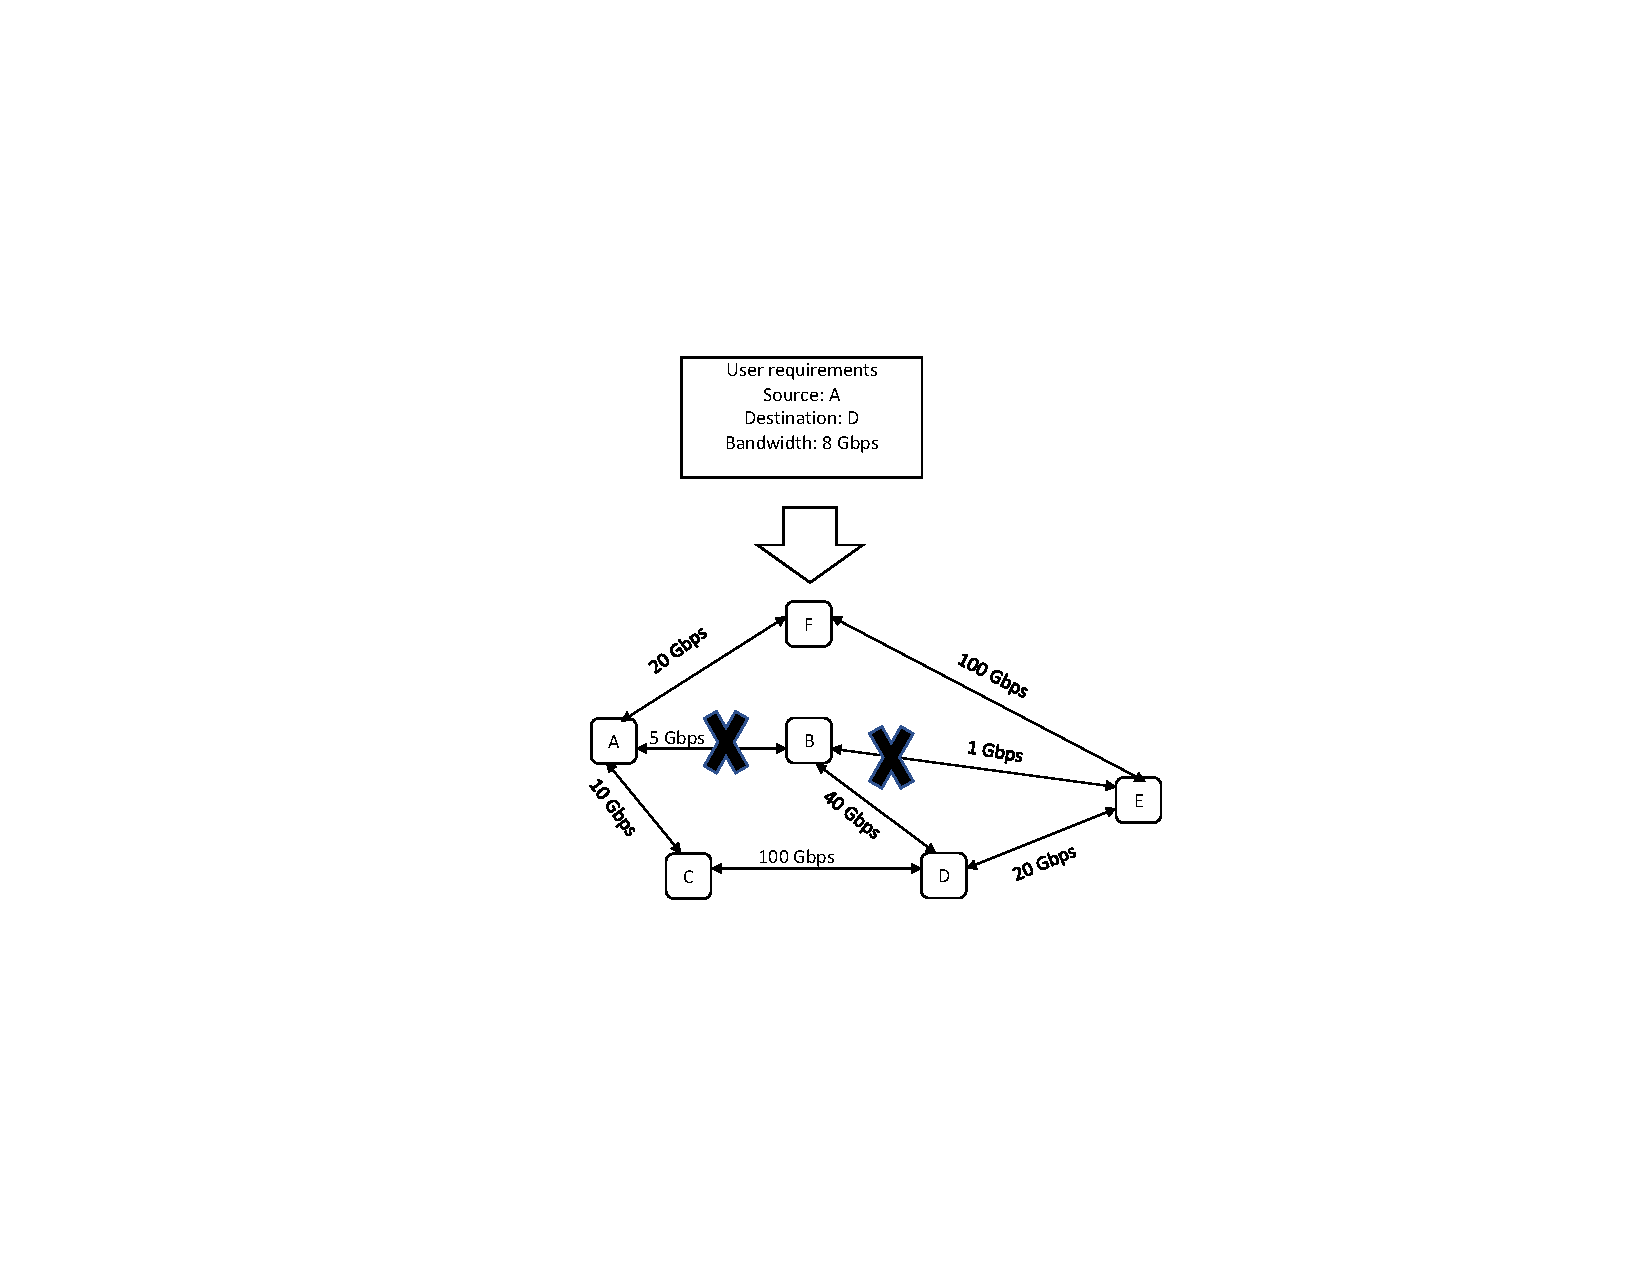
\includegraphics[width=\linewidth, trim= 3.9in 2.3in 3.2in 2.3in, clip]{chapter2/fig1}
		\caption{Pruning}
		\label{fig:pruning}
        \end{subfigure}%
	\hfill
	\begin{subfigure}{0.45\textwidth}\vspace{3em}
        	\centering
		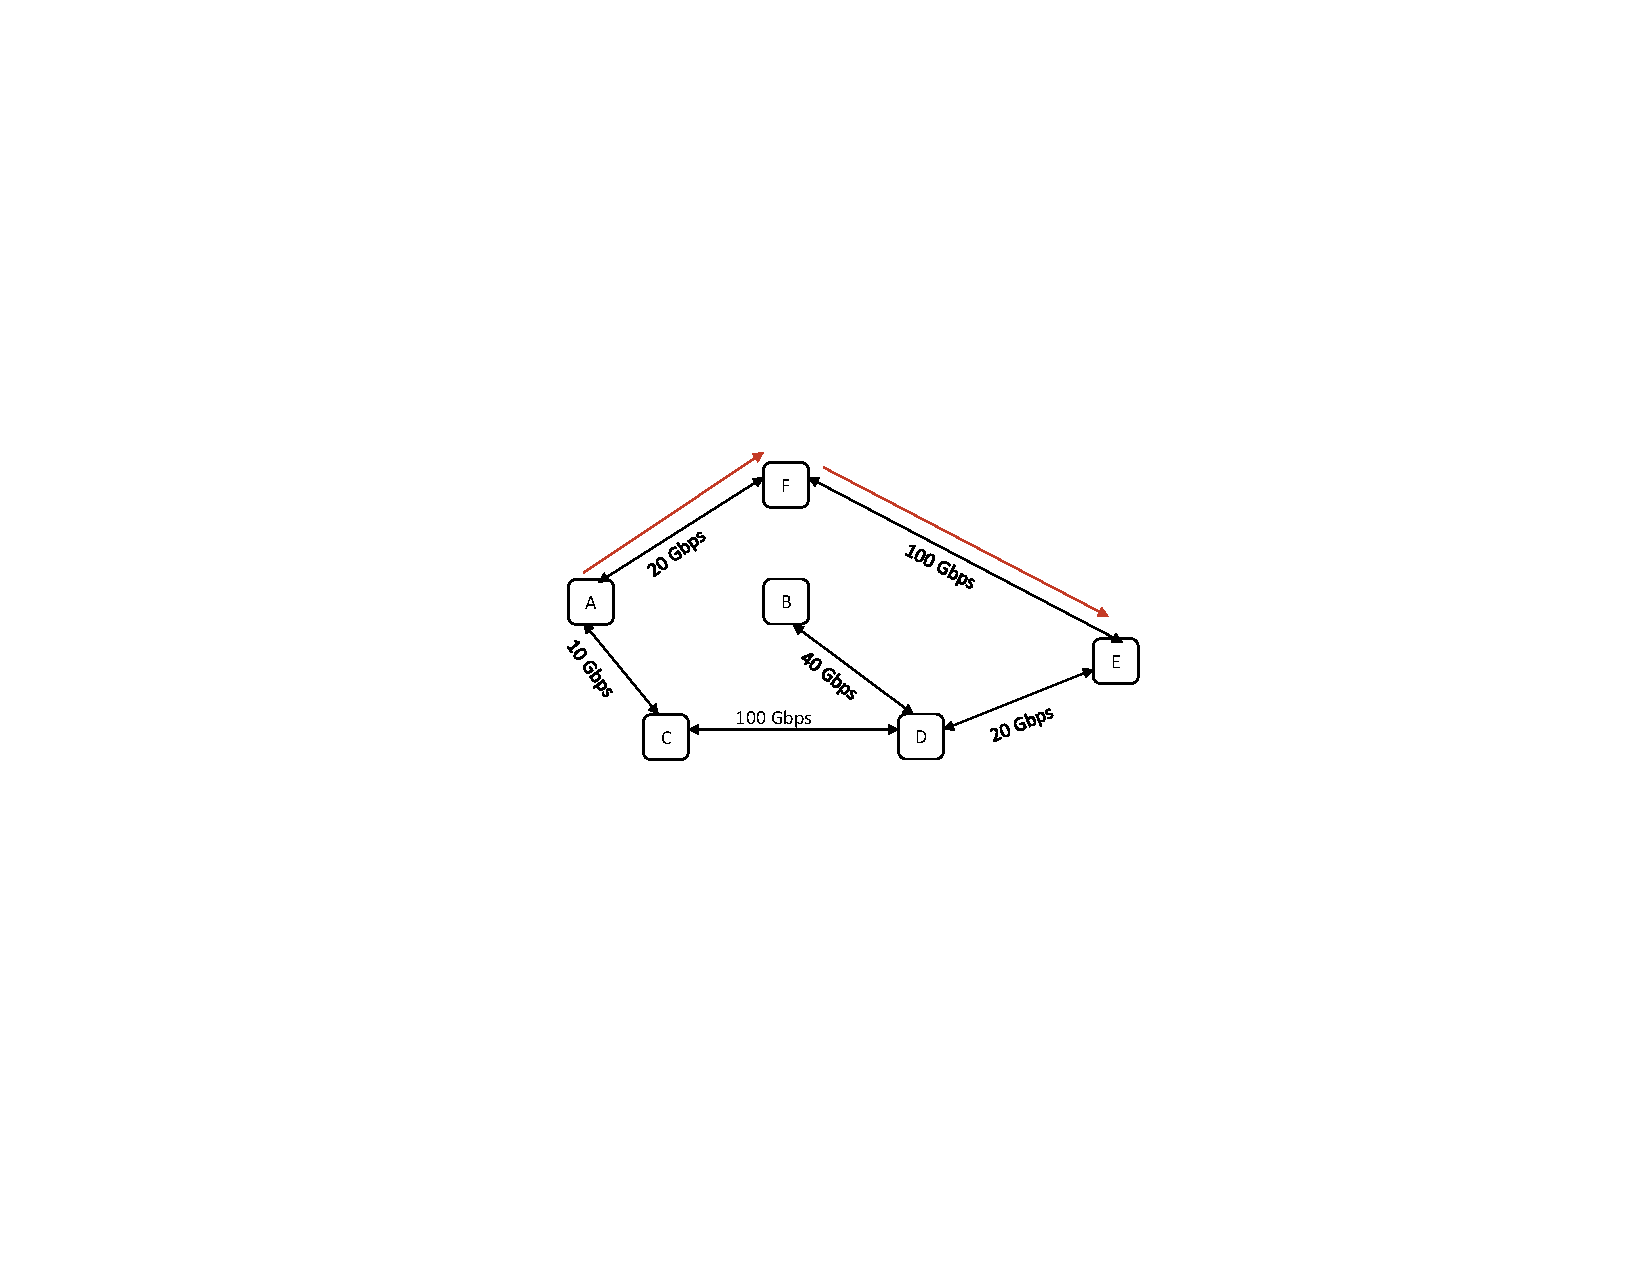
\includegraphics[width=\linewidth, trim = 3.7in 3.2in 3.3in 3.0in, clip]{chapter2/fig2}\vspace{1em}
		\caption{Path Computation}\vspace{-3em}
		\label{fig:pathComputation}
        \end{subfigure}
	\hfill
\caption{Illustration of Basic PCE Service Execution in OSCARS}
\label{fig:basicPCE}
\end{figure*}

%\begin{figure}[H]
%\centering
%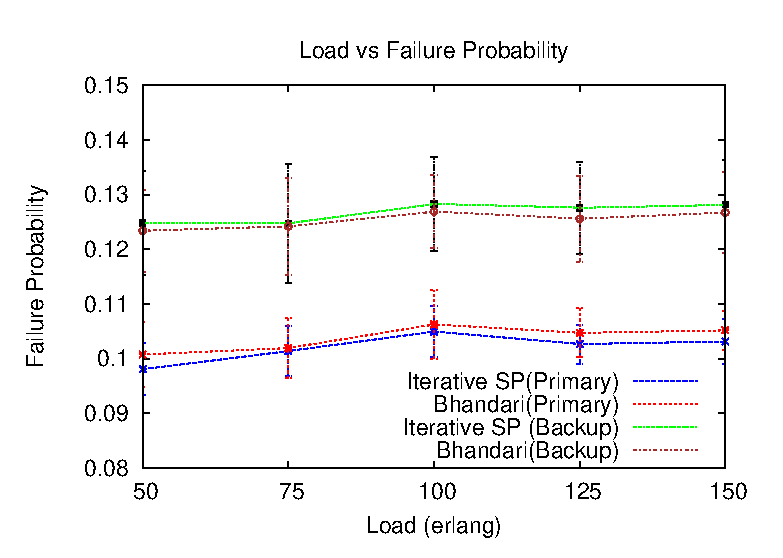
\includegraphics[width=0.75\linewidth]{chapter5/example}
%\caption{Iterative disjoint SP Vs Bhandari - Blocking}
%\label{fig:iterVsBhBlock}
%\end{figure}

\subsubsection{Path computation}

The Path-Computation Element (PCE) in OSCARS v1.0 is built on a uniquely flexible framework that allows distinct path computation elements to be composed an arbitrary workflow sequence.  There are more PCE components than previous versions of OSCARS, added to the OSCARS v1.0 prototype along with their offered service enhancements and algorithms to find the solution path. Prior to pathfinding, the pruning services should be employed to remove the links, ports that cannot support requested bandwidth and vlan tags. Then these PCE's employ low level pathfinding algorithms to compute least-cost path between two nodes. In this research, we are going to utilize these low level pathfinding algorithms for our survivable connection analysis. 

\subsection{Services offered by PCE}
The following subsection only discusses the services offered by PCE components that are applied in this research. Other services can be found at [].

\subsubsection{Unicast Service}
Unicast routing is the process of finding a path between two nodes, sender and receiver. This is the only service offered by the previous version of OSCARS and will be supported in the OSCARS v1.0. It is one of the basic services offered by PCE to compute the shortest path between two nodes in the pruned network. The shortest path can be computed by invoking Dijkstra [geeks] path finding module. Note that this is not the shortest route on the network but rather the shortest working solution after pruning. 

\subsubsection{Anycast Service}
Anycast routing is very similar to unicast routing except that sender node has option of setting up the connection with one of the specified receiver nodes. This can be decided by anycast degree. Anycast degree is the number of optional receiver nodes. It starts by finding a shortest least cost paths to each node one by one. Then it compares the cost of obtained shortest paths and picks the one with least cost path. In figure 2.3, Sender can set up a connection with either E or F. It selects E over F because its the least-cost path. Anycast also employs Dijkstra to find the shortest path

\subsubsection{Palindromic service}
Palindrome, as the name implies, should have both the forward and reverse paths same. Previous versions of OSCARS supports only palindrome. But OSCARS v1.0 introduces 'Non-palindrome' that allows both the forward and reverse path to be different. Figure 2.4 discusses this difference with an example. Figure 2.4(a) explains how the connection is not possible with palindrome but possible with Non-palindrome in Figure 2.4(b). This research analyzed the impact of palindromic connections for failure and blocking.

In figure 2.4 (a), once the links are pruned, there are no paths between A and F. This is because of pruning. Once a request for ? bw arrives, it removes both the inbound and outbound links even if one of them could not support requested bandwidth. However, with Non-palindrome option, it can set up connection successfully because it prunes either only the inbound or outbound that could not support the requested bandwidth.  

\subsubsections{Survivability service}
This service incorporates link-disjoint survivable routing of backup paths. The connection request may be for any number of disjoint paths and the obtained solution paths are assigned identical bandwidths. The only path finding algorithm in OSCARS v1.0 for survivability is Bhandari's link disjoint algorithm. This will be discussed in the section ?

\subsections{Request and Response Specifications}
OSCARS v1.0 allows user to interact to get information regarding the connection requirements through an API. The research makes use of this API [www.mulesoft.com] to submit connection requests to OSCARS. On receiving the request OSCARS processes them and responds with successful or unsuccessful reservation objects. The response object also returns the associated path if successful. Figure 2.5 illustrates the high level view of how the requests can be submitted to OSCARS to get the response.

Table 2.1, 2.2 discusses some of the important request specifications and response. 
%table 1,2
\begin{table}[hbt!]
\centering
\caption{Input Request Specifications}
 	\begin{tabular}{|c|m{24em}|}
	\hline\hline
	\textbf{Parameter} & \textbf{Description} \\
	\hline
	Connection ID&Unique ID for a connection request\\
	\hline
	Start time&Starting time of a connection request\\
	\hline
	End time&This is the time that reserved circuits for this connection get released\\
	\hline
	Source Node&Sending node for this connection\\
	\hline
	Destination Node&Receiving node for this connection\\
	\hline
	Source Port&Source port in a selected source node\\
	\hline
	Destination Port&Destination port in a selected destination node\\
	\hline
	AZ Bandwidth& Forward path bandwidth for the end to end connection request\\
	\hline
	ZA Bandwidth& Reverse Path Bandwidth for the end to end connection request\\
	\hline
	Palindromic&Decides if Forward and Reverse paths are same based on binary value\\
	\hline
	Blacklist&Nodes and Ports to be pruned before finding path. Note that this is different from the pruning due to insufficient link or port bandwidth and vlan tags.\\
	\hline
	Number of Paths&The number of disjoint backup paths for the connection\\
	\hline
	\end{tabular}
\end{table}

\begin{table}[hbt!]
\centering
\caption{Response Parameters}
 	\begin{tabular}{|c|c|}
	\hline\hline
	\textbf{Parameter} & \textbf{Description} \\
	\hline
	Connection ID&Identification of a connection request\\
	\hline
	Status&Status of connection request (Successful or Unsuccessful)\\
	\hline
	Path&Forward and Reverse path for the connection\\  
	\hline
	\end{tabular}
\end{table}


\section Survivable algorithms 

The survivability of a connection can be realized through physical diversity. This can be achieved by setting up a connection with two or more disjoint paths. The term 'Disjoint' in itself can be either node or just link disjoint. Fortunately, there are algorithms that can run in polynomial time to find node/link disjoint paths (K$>$=1) where, K is the number of backup paths. In this research, we are considering two common link-disjoint algorithms, iterative Dijkstra and Bhandari for their performances against considered performance metrics. These performance metrics are briefly explained in chapter 5. In this section, we are going to discuss how they can be implemented for survivable paths.
 
\subsubsection{Iterative Shortest Path}
This algorithm runs Dijkstra twice to find two disjoint paths. It is simple and straightforward but not a part of OSCARS v1.0. By making use of input specifier 'Blacklists' which prunes the specified links and nodes temporarily, it is possible to perform this algorithm with the help of OSCARS v1.0. Figure 2.6 illustrates the implementation steps one by one with the help of OSCARS.

\begin{enumerate}[leftmargin=*,label=(\alph*)]
\item Finds the shortest path with Dijkstra
\item Removes the links in first shortest path from the network with the help of input specifier 'Blacklist' and run Dijkstra again
\item This results in two disjoint paths between a source and destination node.
\end{enumerate}


\begin{figure*}[hbt!]
\centering
      	\begin{subfigure}{0.32\textwidth}
	\centering
		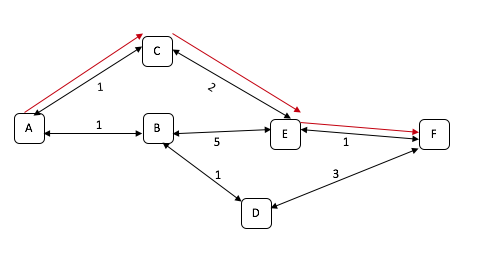
\includegraphics[width=6cm, height=6cm]{chapter2/fig8}
		\caption{}
		\label{fig:ispa1}
        \end{subfigure}%
	\hspace{30mm}
	\begin{subfigure}{0.32\textwidth}
        	\centering
		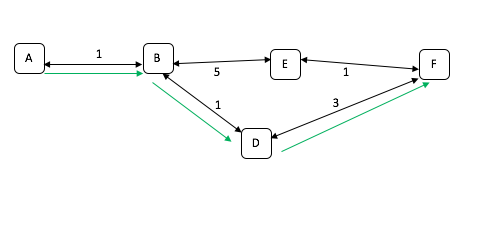
\includegraphics[width=6cm, height=6cm, clip]{chapter2/fig9}
		\caption{}
		\label{fig:ispa2}
        \end{subfigure}
	\vfill
	\begin{subfigure}{0.32\textwidth}
        	\centering
		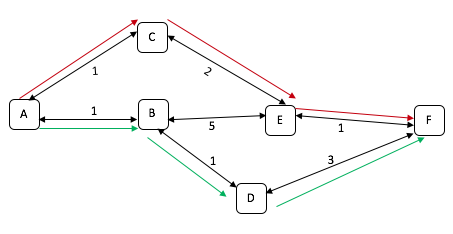
\includegraphics[width=6cm, height=6cm, clip]{chapter2/fig10}
		\caption{}
		\label{fig:ispa3}
        \end{subfigure}
\caption{Iterative Disjoint Shortest path Algorithm}
\label{fig:ispAlgo}
\end{figure*} 

To set up a survivable connection with iterative Dijkstra, one has to contact OSCARS twice.

\subsubsection{Problem with iterative Dijkstra}
\indent Figure 2.7 illustrates the possible scenario where iterative Dijkstra could not find disjoint-backup path although there exists two disjoint-paths. Dijkstra greedily tries to allocate minimum resources as possible to the primary path and fails to set up the backup path(s). See figure 2.7.
%figure 2.7
\begin{figure*}[hbt!]
\centering
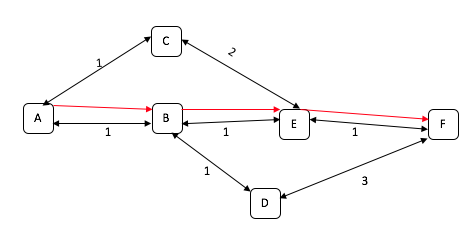
\includegraphics[width=8cm, height=8cm]{chapter2/fig11}
\caption{Problem with iterative SP approach}
\label{fig:problemInIspa}
\end{figure*}

\indent In figure 2.7, you can find only one path between A-F although there are two disjoint paths from A-C-E-F and A-B-D-F. Since, it takes the shortest cost path A-B-E-F, it cannot successfully set up the survivable connection.


\subsubsection{Bhandari's link disjoint} 
Above problem can be overcome with link-disjoint path algorithm, Bhandari. It is based on Suurballe's node-disjoint [www.macfreek.nl] algorithm. Note that Suurballe's requirement is comparatively stricter than Bhandari's as it does not allow primary-backup path pairs to share any node. Although Bhandari has some implementation benefits because it's simpler and faster. OSCARS v1.0 is packaged with a native Bhandari module to support disjoint solutions. 

This algorithm runs on top of single source shortest path algorithms Dijkstra (works only with positive edge weights) and Bellmann ford [www.brilliant.org] (variation of Dijkstra that works with negative edge weights). These heuristics have been extensively utilized in network route establishments for decades. Figure 2.8 explains how Bhandari finds two shortest edge-disjoints paths between A and F. Note that this is the same network graph that iterative Dijkstra fails to compute primary-backup path pair.

\begin{enumerate}[leftmargin=*,label=(\alph*)]
\item Find the shortest path with Dijkstra
\item Reverse the edges of that shortest path with negative costs and once again runs the shortest path algorithm but this time Bellman Ford due to the introduction of negative edge costs
\item Removes the inverse edges obtained from the two paths
\item Bring back all the edges from the two paths, you can get two disjoint paths
\end{enumerate}

%figure 
\begin{figure*}[!hbt]
\centering
      	\begin{subfigure}{0.32\textwidth}
	\centering
		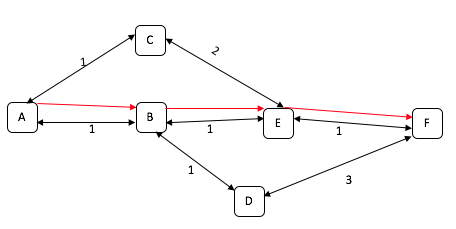
\includegraphics[width=6cm, height=6cm]{chapter2/fig4}
		\caption{}
		\label{fig:bhandari1}
        \end{subfigure}%
	\hspace{30mm}
	\begin{subfigure}{0.32\textwidth}
        	\centering
		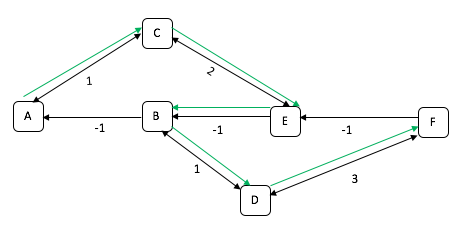
\includegraphics[width=6cm,height=6cm, clip]{chapter2/fig5}
		\caption{}
		\label{fig:bhandari2}
        \end{subfigure}
\vspace{5mm}
      	\begin{subfigure}{0.32\textwidth}
	\centering
		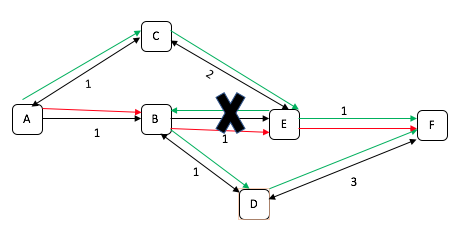
\includegraphics[width=6cm, height=6cm]{chapter2/fig6}
		\caption{}
		\label{fig:bhandari3}
        \end{subfigure}%
	\hspace{30mm}
	\begin{subfigure}{0.32\textwidth}
        	\centering
		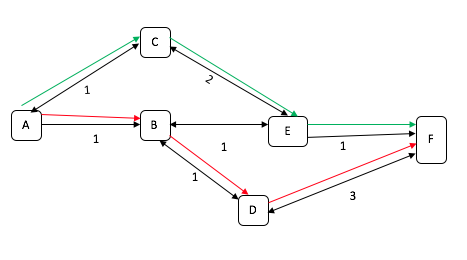
\includegraphics[width=6cm, height=6cm, clip]{chapter2/fig7}
		\caption{}
		\label{fig:bhandari4}
        \end{subfigure}
	\hfill
\caption{Bhandari's Disjoint Path Pair Algorithm}
\label{fig:bhandari}
\end{figure*}
                                                              

\indent After obtaining the two disjoint paths, one would like to consider the shortest cost path as the primary or working path. The advantage of Bhandari is that it tries to find the total optimal cost and distribute amongst the paths. In other words, it's not greedy as Djikstra and hence, it can find disjoint-paths almost all the time if there is one. Hence, Bhandari is an excellent solution for protection scenario since the connections are set in advance. 
